
\ccUserChapter{Kinetic Data Structures}
\label{chapter-kds}
\ccChapterAuthor{Daniel Russel}


\begin{ccPkgDescription}{3D Convex Hulls\label{Pkg:ConvexHull3}}
\ccPkgHowToCiteCgal{cgal:hs-ch3-07}
\ccPkgSummary{This package provides functions 
for computing convex hulls in three dimensions as well as functions
for checking if sets of points are strongly convex are not. One can
compute the convex hull of a set of points in three dimensions in one
of three ways: using a static algorithm, using an incremental
construction algorithm, or using a triangulation to get a fully
dynamic computation.}

\ccPkgDependsOn{All algorithms produce as output a \ccRef[3D Polyhedron]{Pkg:Polyhedron}. 
                The dynamic algorithms depend on \ccRef[3D Triangulations]{Pkg:Triangulation3}}
\ccPkgIntroducedInCGAL{1.1}
\ccPkgLicense{\ccLicenseQPL}
\ccPkgIllustration{Convex_hull_3/bunny.png}{Convex_hull_3/bunny.png}
\end{ccPkgDescription}


\minitoc


\ccDefGlobalScope{CGAL::}

\def\note#1{$\langle\langle${\bf #1}$\rangle\rangle$}
%\message{Remove note before final version!}
%\def{\th}{^{\rm th}}

% space tweaks
%\addtolength{\parskip}{-1pt}

%\section{Todo}

\subsection{General thoughts}

\begin{itemize}

\item there might be a bug in Simple_interval_root due to its use of
  approximate_interval_width (which uses doubles and so might never
  get small enough).

\item The other trajectory modification events need to be documented
  (Set\_moving\_point). Hmmm, I don't remember what this means. 

\item There is no 2d regular triangulation. This is not too much work,
  but a bit (since I will need to refactor my 2d delaunay)

\item the FunctionKernel is not documented much (the options are never
  explained)

\item The is some confusion about where a KDS should get a
  FunctionKernel. Currently they mostly get them from the Simulator
  (which directly provides the RootStack). I am not sure that this is
  the right solution. The better solution may just be to have the
  FunctionKernel (and RootStack) be fetched from the SimulationTraits.

\item The FunctionKernel numeric solver I implemented is not as good
  as the one provided by GSL which is shipped on most linux boxes. It
  is GPL, so the user does have to make a decision about using it.
  Currently, there is a traits class that the user can select if they
  want to use it (at the cost of reassembling the SimulationTraits).

\item The 3d visualizion uses Coin. It is currently all in headers so
  there is really no problem with the user only using it if they have
  coin. It is pretty simple to port it to any other 3d viewer if CGAL
  picks one.

\item The whole SimulationTraits is a bit funny since it allows you to
  a) fetch a bunch of kernels and b) fetch pointers to the
  ActiveObjectsTable and simulator. I don't see an obvious way to keep
  its simplicity and have it make more sense.

\item the Qt stuff is broken since I am waiting for the proper person
  to update the makefile


\end{itemize}

%%% Local Variables: 
%%% mode: latex
%%% TeX-master: t
%%% End: 


Lets say you want to maintain a sorted list of items (each item is
associate with a real number key). You can imagine placing each of the
items on the point on the real line corresponding to its key. Now, let
the key for each item change continuously (i.e. no jumps are allowed).
As long as no to (consecutive) items cross, the sorted order is
intact. When two cross, they need to be exchanged in the list and then
the sorted order is once again correct. This is a trivial example of a
kinetic data structure. The key observation is that the combinatorial
structure which is maintained changes at discrete times (events) even
though the basic building blocks are changing continuously.

This chapter describes a framework for implementing kinetic data
structures and sweepline algorithms as well as several kinetic data
structures implemented on top of this framework. The framework was
first presented at ALENEX~\cite{cgal:gkr-cfhm-04}. We first, in
Section~\ref{sec:kds_intro} introduce kinetic data structures and
sweepline algorithms. This section can be skipped if the reader is
already familiar with the area. The next sections,
Section~\ref{sec:kds_terms} and Section~\ref{sec:overview} introduces
the terms and gives an overview of the framework. They are recommended
reading for all readers. We then present kinetic data structures for
Delaunay triangulations in two and three dimensions in
Section~\ref{sec:provided_kdss}. Following that, in
Section~\ref{sec:architecture} we discuss the architecture of the
framework and finally we give several examples of using the framework
to implement a kinetic data structure in
Section~\ref{sec:examples}. The framework makes heavy use of our
\ccc{Polynomial_kernel} package to provide models of the
\ccc{Kinetic::FunctionKernel} concept.

%%%%%%%%%%%%%%%%%%%%%%%%%%%%%%%%%%%%%%%%%%%%%%%%%%%%%%%%%%%%%%%%%%%%
\section{Kinetic Data Structures and Sweep Algorithms}
\label{sec:kds_intro}
%%%%%%%%%%%%%%%%%%%%%%%%%%%%%%%%%%%%%%%%%%%%%%%%%%%%%%%%%%%%%%%%%%%%


\subsection{Kinetic Data Structures}
Kinetic data structures were first introduced in by Basch et.\ al.\ in
1997~\cite{cgal:bgh-dsmd-97}.  The idea stems from the observation that
most, if not all, computational geometry structures are built using
{\em predicates} --- functions on quantities defining the geometric
input (e.g.\ point coordinates), which return a discrete set of
values. Many predicates reduce to determining the sign of a polynomial
on the defining parameters of the primitive objects. For example, to
test whether a point lies above or below a plane we compute the dot
product of the point with the normal of the plane and subtract the
plane's offset along the normal. If the result is positive, the point
is above the plane, zero on the plane, negative below. The validity of
many combinatorial structures built on top of geometric primitives can
be verified by checking a finite number of predicates of the geometric
primitives.  These predicates, which collectively certify the
correctness of the structure, are called {\em certificates}.  For a
Delaunay triangulation in three dimensions, for example, the
certificates are one \ccc{InCircle} test per facet of the
triangulation, plus a point plane orientation test for each facet or
edge of the convex hull.

The kinetic data structures approach is built on top of this view of
computational geometry. Let the geometric primitives move by replacing
each of their defining quantities with a function of time (generally a
polynomial). As time advances, the primitives trace out paths in
space called {\em trajectories}. The values of the polynomial
functions of the defining quantities used to evaluate the predicates now
also become functions of time. We call these functions
{\em certificate functions}. Typically, a geometric structure is valid when
all predicates have a specific non-zero sign. In the kinetic setting,
as long as the certificate functions maintain the correct sign as time varies,
the corresponding predicates do not change values,
and the original data structure remains correct. However, if
one of the certificate functions changes sign, the original structure
must be updated, as well as the set of certificate functions that
verify it.  We call such occurrences {\em events}.

Maintaining a kinetic data structure is then a matter of determining
which certificate function changes sign next, i.e.\ determining which
certificate function has the first real root that is greater than the
current time, and then updating the structure and the set of
certificate functions. In addition, the trajectories of primitives are
allowed to change at any time, although $C^0$-continuity of the
trajectories must be maintained.  When a trajectory update occurs for
a geometric primitive, all certificates involving that primitive must
be updated.  We call the collection of kinetic data structures,
primitives, event queue and other support structures a
{\em simulation}.

Sweepline algorithms for computing arrangements in $d$ dimensions
easily map on to kinetic data structures by taking one of the
coordinates of the ambient space as the time variable. The kinetic
data structure then maintains the arrangement of a set of objects
defined by the intersection of a hyperplane of dimension $d-1$ with
the objects whose arrangement is being computed. 


Time is one of the central concepts in a kinetic simulation.  Just as
static geometric data structures divide the continuous space of all
possible inputs (as defined by sets of coordinates) into a discrete
set of combinatorial structures, kinetic data structures divide the
continuous time domain into a set of disjoint intervals. In each
interval the combinatorial structure does not change, so, in terms of
the combinatorial structure, all times in the interval are equivalent.
We capitalize on this equivalence in the framework in order to
simplify computations. If the primitives move on polynomial
trajectories and the certificates are polynomials in the coordinates,
then events occur at real roots of polynomials of time. Real numbers,
which define the endpoints of the interval, are more expensive to
compute with than rational numbers, so performing computations at a
rational number inside the interval is preferable whenever
possible. See Section~\ref{instantaneous_kernel} for an example of
where this equivalence is exploited.

%%%%%%%%%%%%%%%%%%%%%%%%%%%%%%%%%%%%%%%%%%%%%%%%%%%%%%%%%%%%%%%%%%%%
\section{Terms Used}
\label{sec:kds_terms}
%%%%%%%%%%%%%%%%%%%%%%%%%%%%%%%%%%%%%%%%%%%%%%%%%%%%%%%%%%%%%%%%%%%%

\begin{description}
\item[primitive] The basic geometric types--i.e.\ the points of a
  triangulation. A primitive has a set of {\em coordinates}.
\item[combinatorial structure] A structure built on top of the
  primitives. The structure does not depend directly on the
  coordinates of the primitives, only on relationships between them.
\item[trajectory] The path traced out by a primitive as time passes.
  In other words how the coordinates of a primitive change with time.
\item[snapshot] The position of all the primitives at a particular
  moment in time.
\item[static] Having to do with geometric data structures on
  non-moving primitives.
\item[predicate] A function which takes the coordinates of several
  primitives from a snapshot as input and produces one of a discrete
  set of outputs.
\item[certificate] One of a set of predicates which, when all having
  the correct values, ensure that the combinatorial structure is
  correct.
\item[certificate function] A function of time which is positive when
  the corresponding certificate has the correct value. When the
  certificate function changes sign, the combinatorial structure needs
  to be updated.
\item[event] When a certificate function changes sign and the
  combinatorial structure needs to be updated.
\end{description}


\subsection{Overview}
\label{sec:overview}
The package is structured around five main concepts. See
Figure~\ref{uml_usage} for a schematic of how a kinetic data
structure interacts with the various parts. The main concepts are
 
% MK:: why is there a + before less_x_1_object() ?
% Another thing is that I am not really sure that we really want this
% figure to appear here. I prefer to have it at the end as it was before.
% I leave it up to you to decide this.
\begin{figure}
\begin{ccTexOnly}
\begin{center}
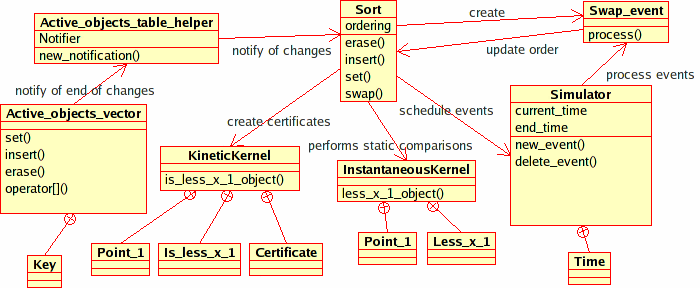
\includegraphics[scale=.8,viewport=0 18 470 250, clip]{Kinetic_data_structures/sort_usage_pct}
\end{center}
\end{ccTexOnly}
\begin{ccHtmlOnly}
<img border=1 src="./sort_usage_pct.gif" align=center alt="Sort Usage"><br>
\end{ccHtmlOnly}
\caption{\label{uml_usage} The figure shows the interaction between
  the \ccc{Kinetic::Sort<Traits, Visitor>} kinetic data structure and
  the various pieces of our package.  Other, more complicated, kinetic
  data structures will also use the \ccc{Kinetic::InstantaneousKernel} in order
  to insert/remove geometric primitives and audit
  themselves. \ccc{Kinetic::Sort<Traits, Visitor>} uses the sorting
  functionality in STL instead.}
\end{figure}

\begin{itemize}

\item the \ccc{Kinetic::Simulator}. Models of this concept process events in
  the correct order and audit kinetic data structures. There should be
  one instance of a model of this concept per simulation.
\item the \ccc{Kinetic::Kernel}. The structure of a
  \ccc{Kinetic::Kernel} is analogous to the static CGAL (i.e.,
  non-kinetic) kernels in that it defines a set of primitives and
  functors which generate certificates from the primitives.
\item the \ccc{Kinetic::ActiveObjectsTable}. Models of this concept hold a
  collection of kinetic primitives in a centralized manner. This
  structure centralizes management of the primitives in order to
  properly disseminate notifications when trajectories change, new
  primitives are added or primitives are deleted.
  There is generally one instance of a model of this concept per simulation.
\item the \ccc{Kinetic::InstantaneousKernel}. Models of this concept allow
  existing non-kinetic CGAL data structures to be used on a snapshot
  of kinetic data. As a result, pre-existing static structures can be
  used to initialize and audit kinetic data structures.
\item the \ccc{Kinetic::FunctionKernel}. This concept is the computational
  kernel of our framework.  Models of this concept are responsible for
  representing, generating and manipulating the motional and
  certificate functions and their roots. It is this concept that
  provides the kinetic data structures framework with the necessary
  algebraic operations for manipulating event times. The
  \ccc{Kinetic::FunctionKernel} is discussed in detail in Section
  \ref{algebraic_kernel}.
\end{itemize}

For simplicity, we added an additional concept, that of
\ccc{Kinetic::SimulationTraits}, which wraps together a particular set of
choices for the above concepts and is responsible for creating
instances of each of the models. The addition of this concept reduces
the choices the user has to make to picking the dimension of the
ambient space and choosing between exact and inexact computations. The
model of \ccc{Kinetic::SimulationTraits} creates an instance each of the
\ccc{Kinetic::Simulator} and \ccc{Kinetic::ActiveObjectsTable}. Handles for
these instances as well as instances of the \ccc{Kinetic::Kernel}
and \ccc{Kinetic::InstantaneousKernel} can be requested from the simulation
traits class. Both the \ccc{Kinetic::Kernel} and the
\ccc{Kinetic::Simulator} use the \ccc{Kinetic::FunctionKernel}, the former to find
certificate failure times and the later to operate on them. For
technical reasons, each supplied model of \ccc{Kinetic::SimulationTraits} also
picks out a particular type of kinetic primitive which will be used by
the kinetic data structures.


% Both the \object{KineticKernel}
%and the \object{Simulator} query the \object{FunctionKernel} for
%constructing certificate functions, as well as getting their failure
%times.

Surrounding these central set of concepts, there are a large number of
smaller concepts, the models of which act either as glue between
objects or as helper classes.  The key smaller concepts will be described along
with the appropriate central concepts in the corresponding subsections
of Section \ref{sec:architecture}.





\section{Using Kinetic Data Structures\label{sec:kds_provided_kdss}}


There are five provided kinetic data structures. They are
\begin{description}
\item[\ccc{Kinetic::Sort<Traits, Visitor>}] maintain a list of points
sorted by x-coordinate.
\item[\ccc{Kinetic::Delaunay_triangulation_2<Traits, Visitor,
    Triangulation>}] maintain the Delaunay triangulation of a set of
  two dimensional points
\item[\ccc{Kinetic::Delaunay_triangulation_3<Traits,Visitor,
    Triangulation>}] maintain the Delaunay triangulation of a set of
  three dimensional points.
\item[\ccc{Kinetic::Regular_triangulation_3<Traits, Visitor,
Triangulation>}] maintain the regular triangulation of a set of waiting
three dimensional points.
\item[\ccc{Kinetic::Enclosing_box_2<Traits>},
  \ccc{Kinetic::Enclosing_box_3<Traits>}] restrict points to stay
  within a box by bouncing them off the walls.
\end{description}


\subsection{Two Dimensional Delaunay}
\label{sec:sort_example}

Using a kinetic data structure can be as simple as the following:
\label{fig:sort_program}
\ccIncludeExampleCode{Kinetic_data_structures/sort.C}

In the example, first the \ccc{Kinetic::SimulationTraits} object is chosen
(in this case one that supports exact computations). Then the kinetic
data structure is defined, using the chosen traits object and a
visitor class which logs changes to the sorted list.  Next, instances
of the two are created and a set of points is read from a file. Then,
the simulator is instructed to process all the events until the end of
the simulation.  Finally, a record of what happened is printed to the
terminal.

Several important things happen behind the scenes in this example.
First, the \ccc{Kinetic::ActiveObjectsTable} which holds the moving points
notifies the kinetic data structure that new points have been added to
the simulation. Second, the \ccc{Kinetic::Sort<Traits,Visitor>} kinetic data structure
registers its events with the \ccc{Kinetic::Simulator} by providing a time
and a proxy object. When a particular event occurs, the
Kinetic::Simulator calls a function on the proxy object which in turn
updates the kinetic data structure.

The example illustrates how to monitor the supplied data structures as
they evolve by using a \ccc{Kinetic::SortVisitor} object---a small class whose
methods are called whenever the kinetic data structure changes. Hooks
for such visitor concepts are provided for all of the shipped kinetic
data structures. In the case of kinetic sorting, the visitor's
methods are called every time a new point is inserted in the sorted
list, when one is removed, or when two points are swapped in the
sorted order. 


The visitor concept is quite powerful, allowing us, for example, to
implement a data structure for computing and storing two-dimensional
arrangements of $x$-monotone curves on top of the
\ccc{Kinetic::Sort<Traits, Visitor>} data structure using about 60
lines of code. This sweepline code is presented in
Section~\ref{sec:sweepline_example}.




\subsection{Two Dimensional Delaunay}
\label{sec:delaunay_2_example}

As with static triangulations, in order to use the data structure the
user must provide a traits class. In addition, an optional visitor
class can be provided to monitor how the data structure changes, and a
custom triangulation can be provided. The traits class must be a model
of \ccc{SimulationTraits}. Most of the details of the traits class can
be ignored for the time being other than two parts 
\begin{description}
\item[\ccc{moving_point_table_pointer()}] this returns a (reference counted) pointer to a table which keeps track of all the primitives.
\item[\ccc{simulator_pointer()}] this returns a pointer to the \ccc{Simulator} which is what controls how time advances.
\end{description}
The framework provides a number of models of the
\ccc{SimulationTraits} named
\{Exact,Inexact\}\_simulation\_traits\_\{1,2,3\}. Here we opt for
exact computations (and require two dimensions).

In order to monitor the Delaunay triangulation as the simulation is
run, we use a visitor. This is a small class, which is passed to the
Delaunay triangulation. The triangulation calls methods on the visitor
class whenever things happen. In the case, the visitor,
\ccc{CGAL::KDS::Delaunay_triangulation_event_log_visitor_2} simply makes a record of each event that occurs.

Once the traits class and kinetic Delaunay have been created, we need
to add points to the simulation. To do this, we add them directly to
the
\ccc{ActiveObjectsTable} using the \ccc{insert} method. 


Now that the triangulation has been set up at points added (or
scheduled for addition), we can run the kinetic data structure. Here
we ask the simulation to process all events and then using the visitor
to print out a record of all events that occur. Note that there are a
finite number of events since eventually all the points are spread far
apart and simply moving outward. If instead, we had added a
\ccc{CGAL::KDS::Enclosing_box_2<Traits>} to the simulation, then 
there would be an infinite number of events as the points repeatedly
bounce off the walls.

For an equivalent example with a graphical interface, see
demo/Kinetic\_data\_structures/Delaunay\_triangulation\_2.C.

\begin{figure*}[htb]
\begin{ccTexOnly}
\begin{center}
1.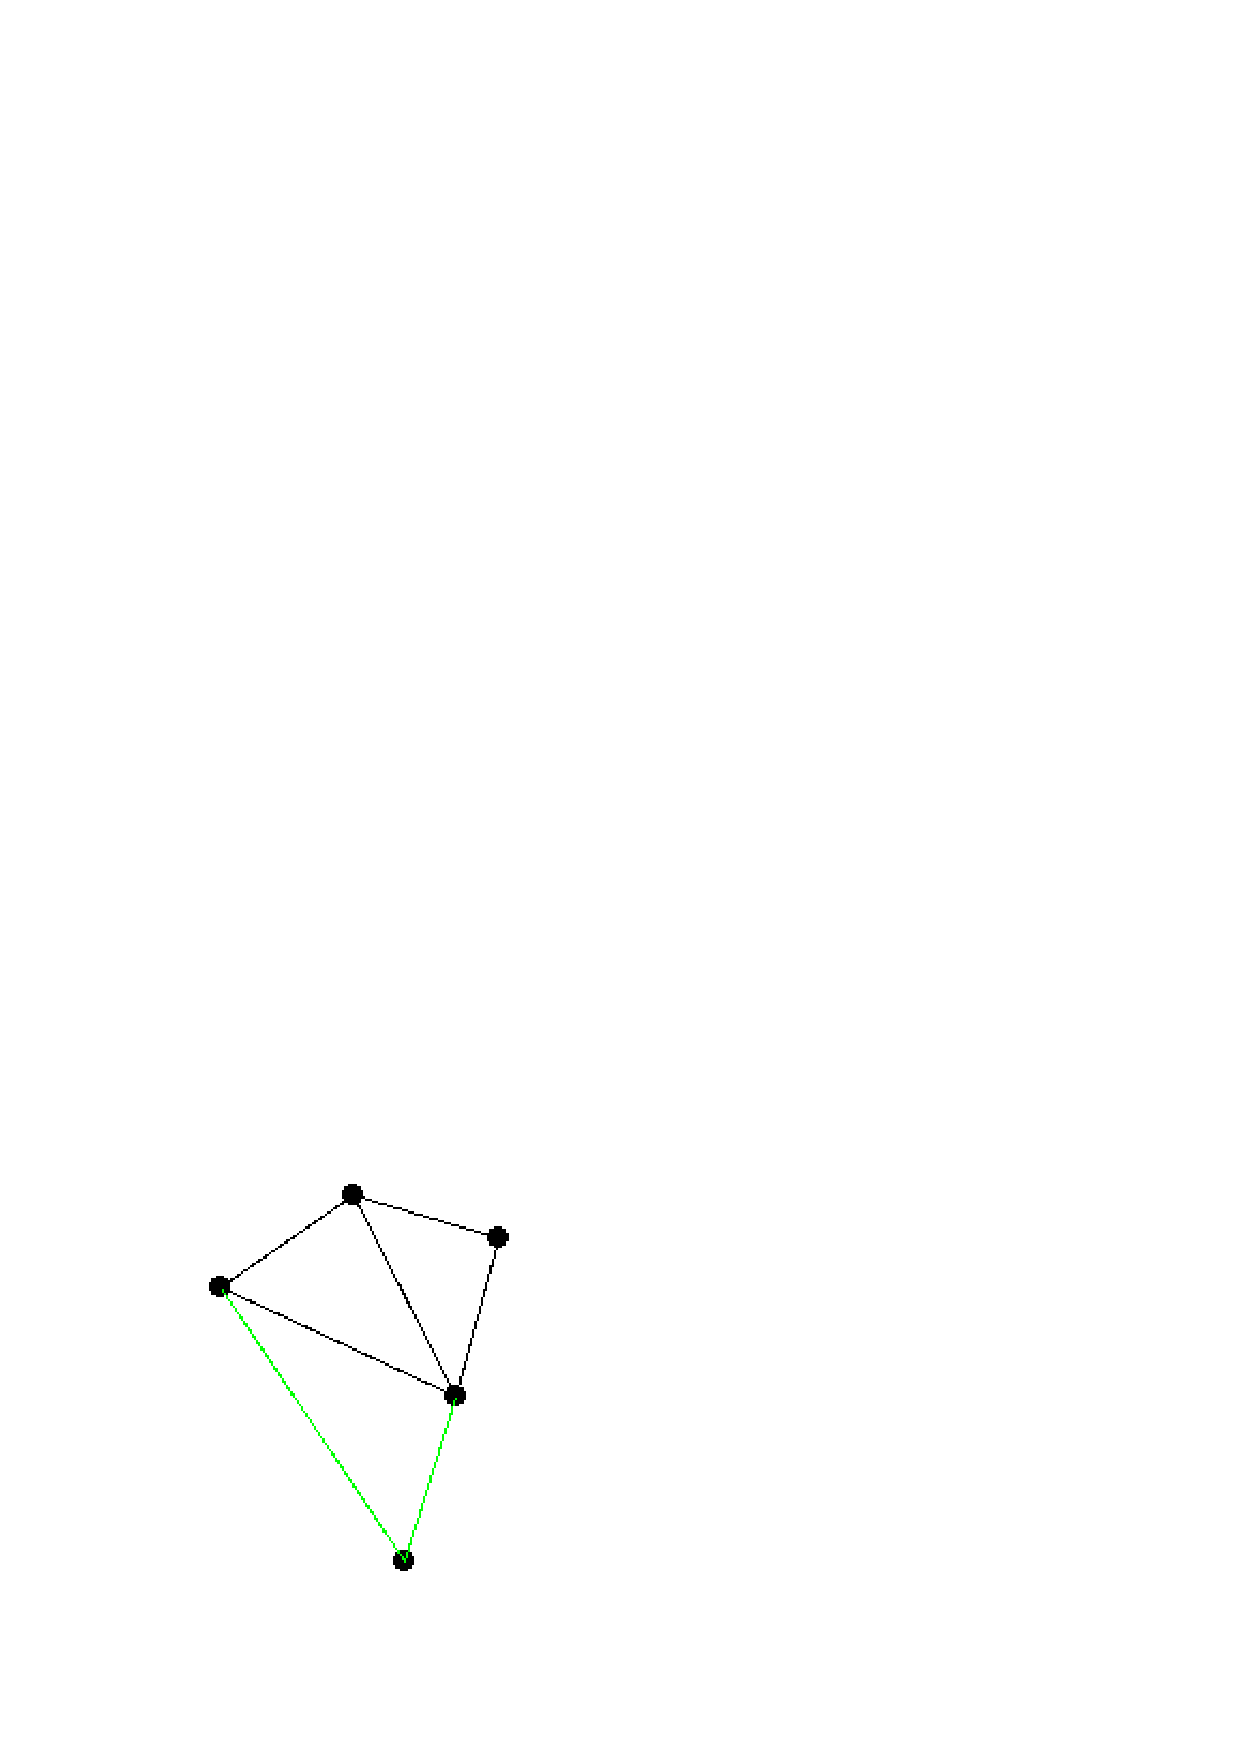
\includegraphics[ scale=.3]{Kinetic_data_structures/delaunay_shot_0_crop_pct} 
2.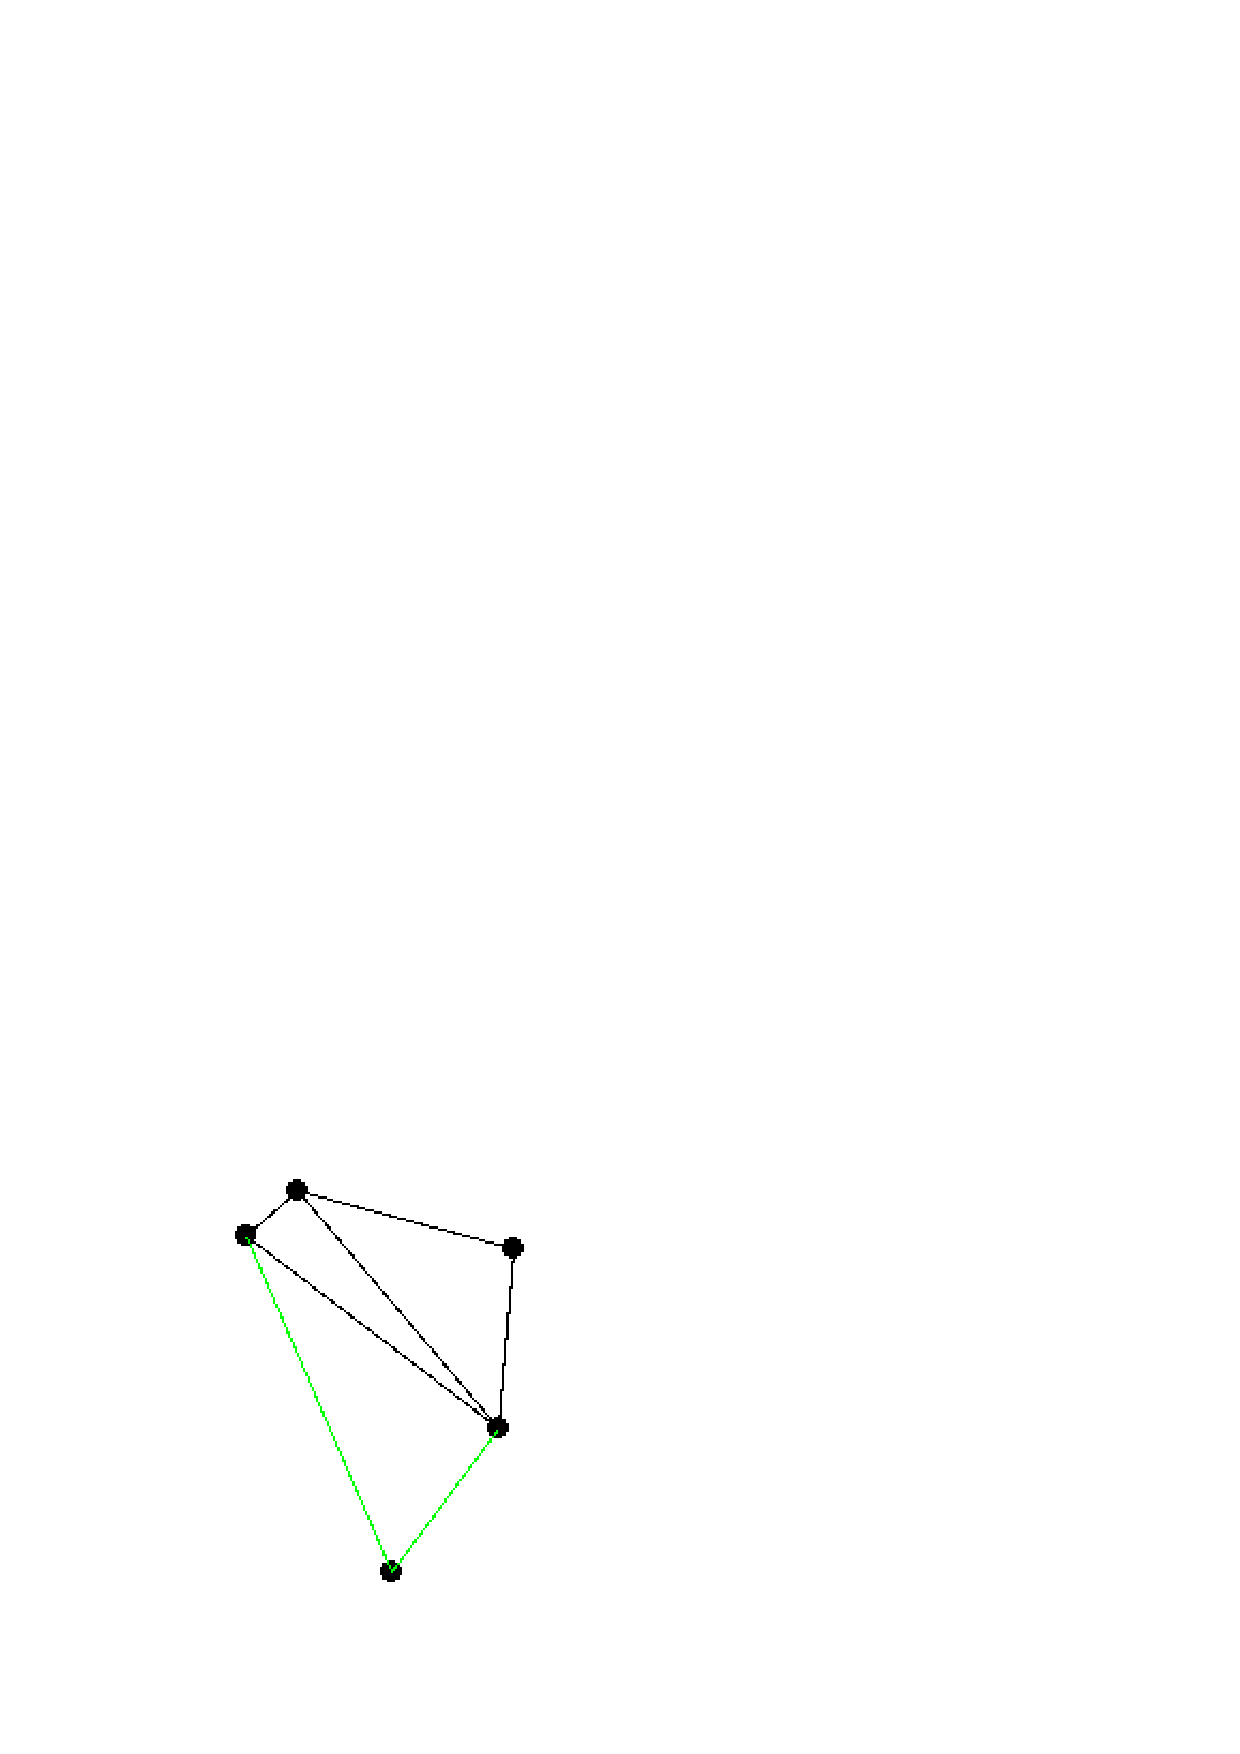
\includegraphics[ scale=.3]{Kinetic_data_structures/delaunay_shot_1_crop_pct}
3.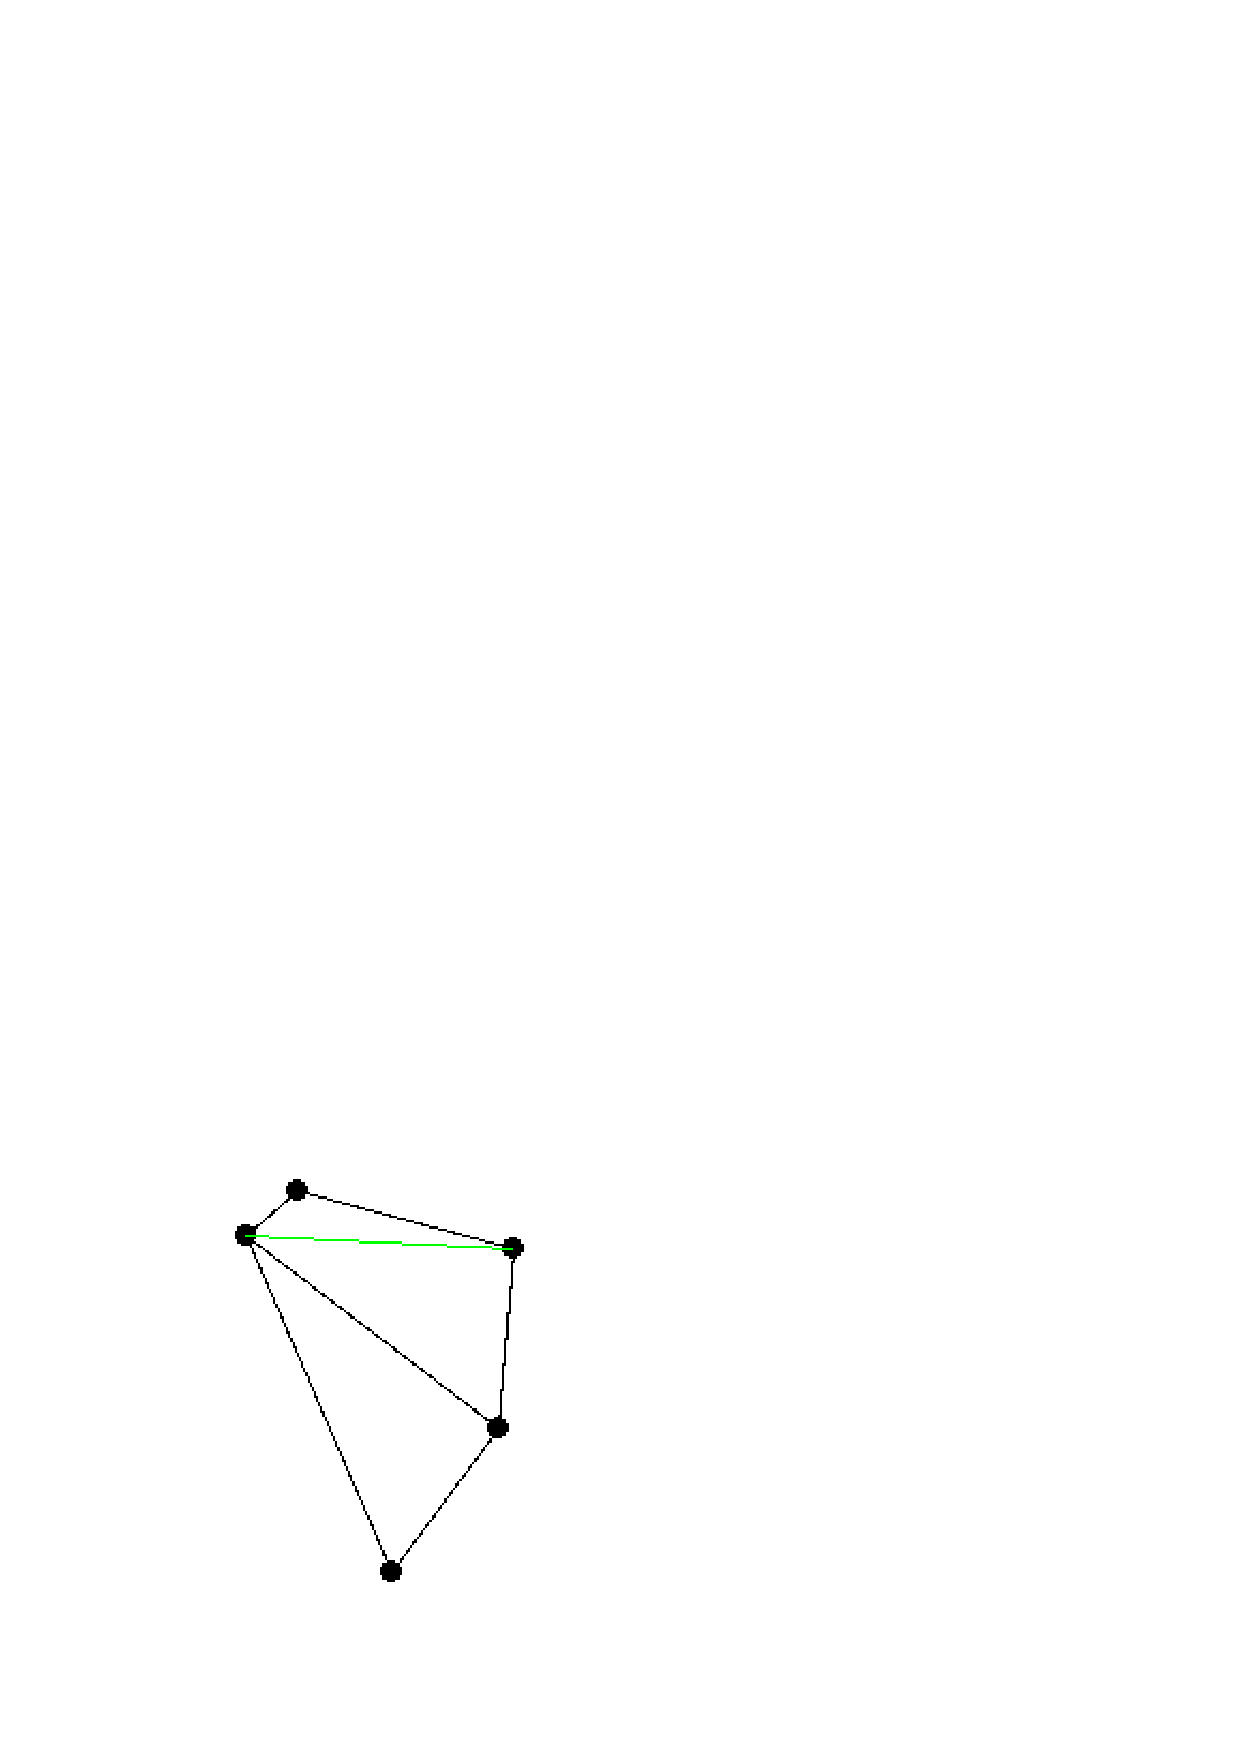
\includegraphics[ scale=.3]{Kinetic_data_structures/delaunay_shot_2_crop_pct}\\
4.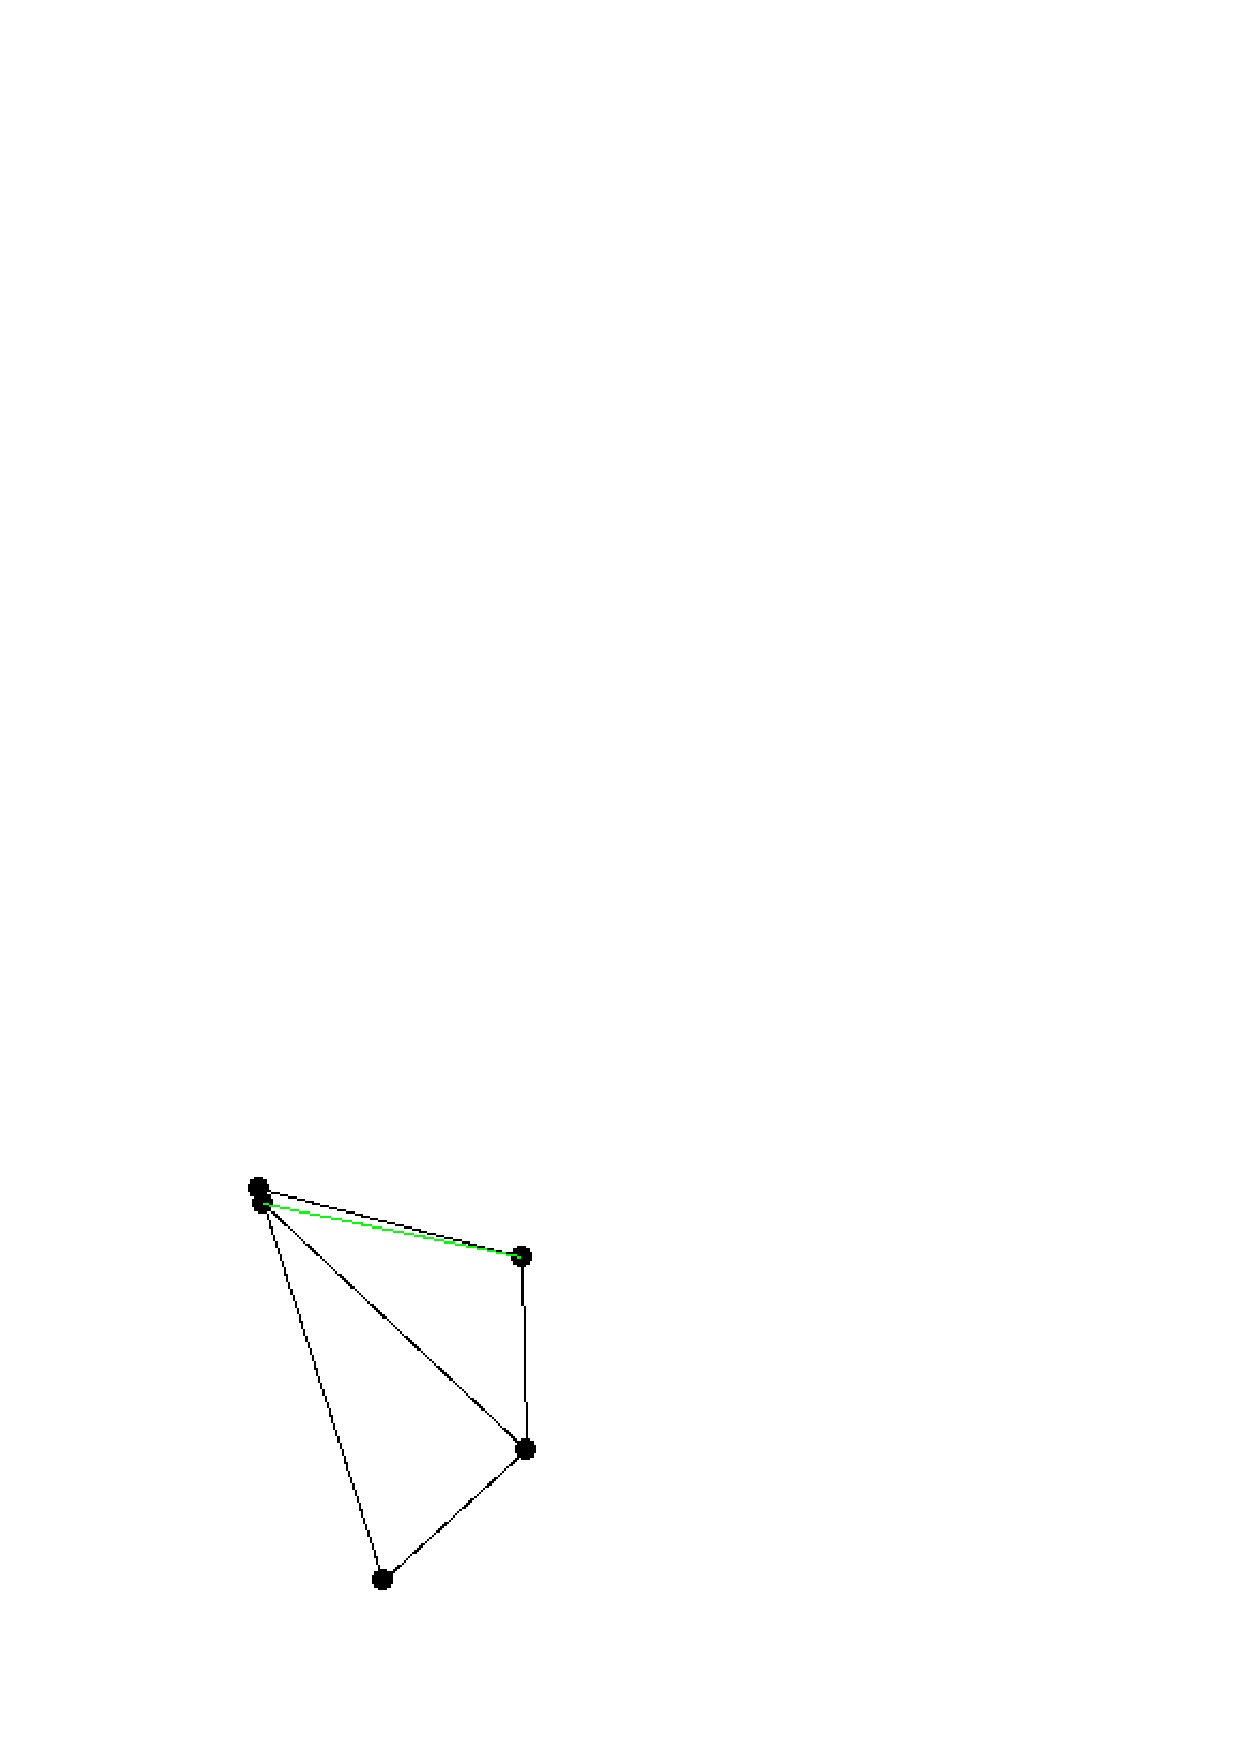
\includegraphics[ scale=.3]{Kinetic_data_structures/delaunay_shot_3_crop_pct}
5.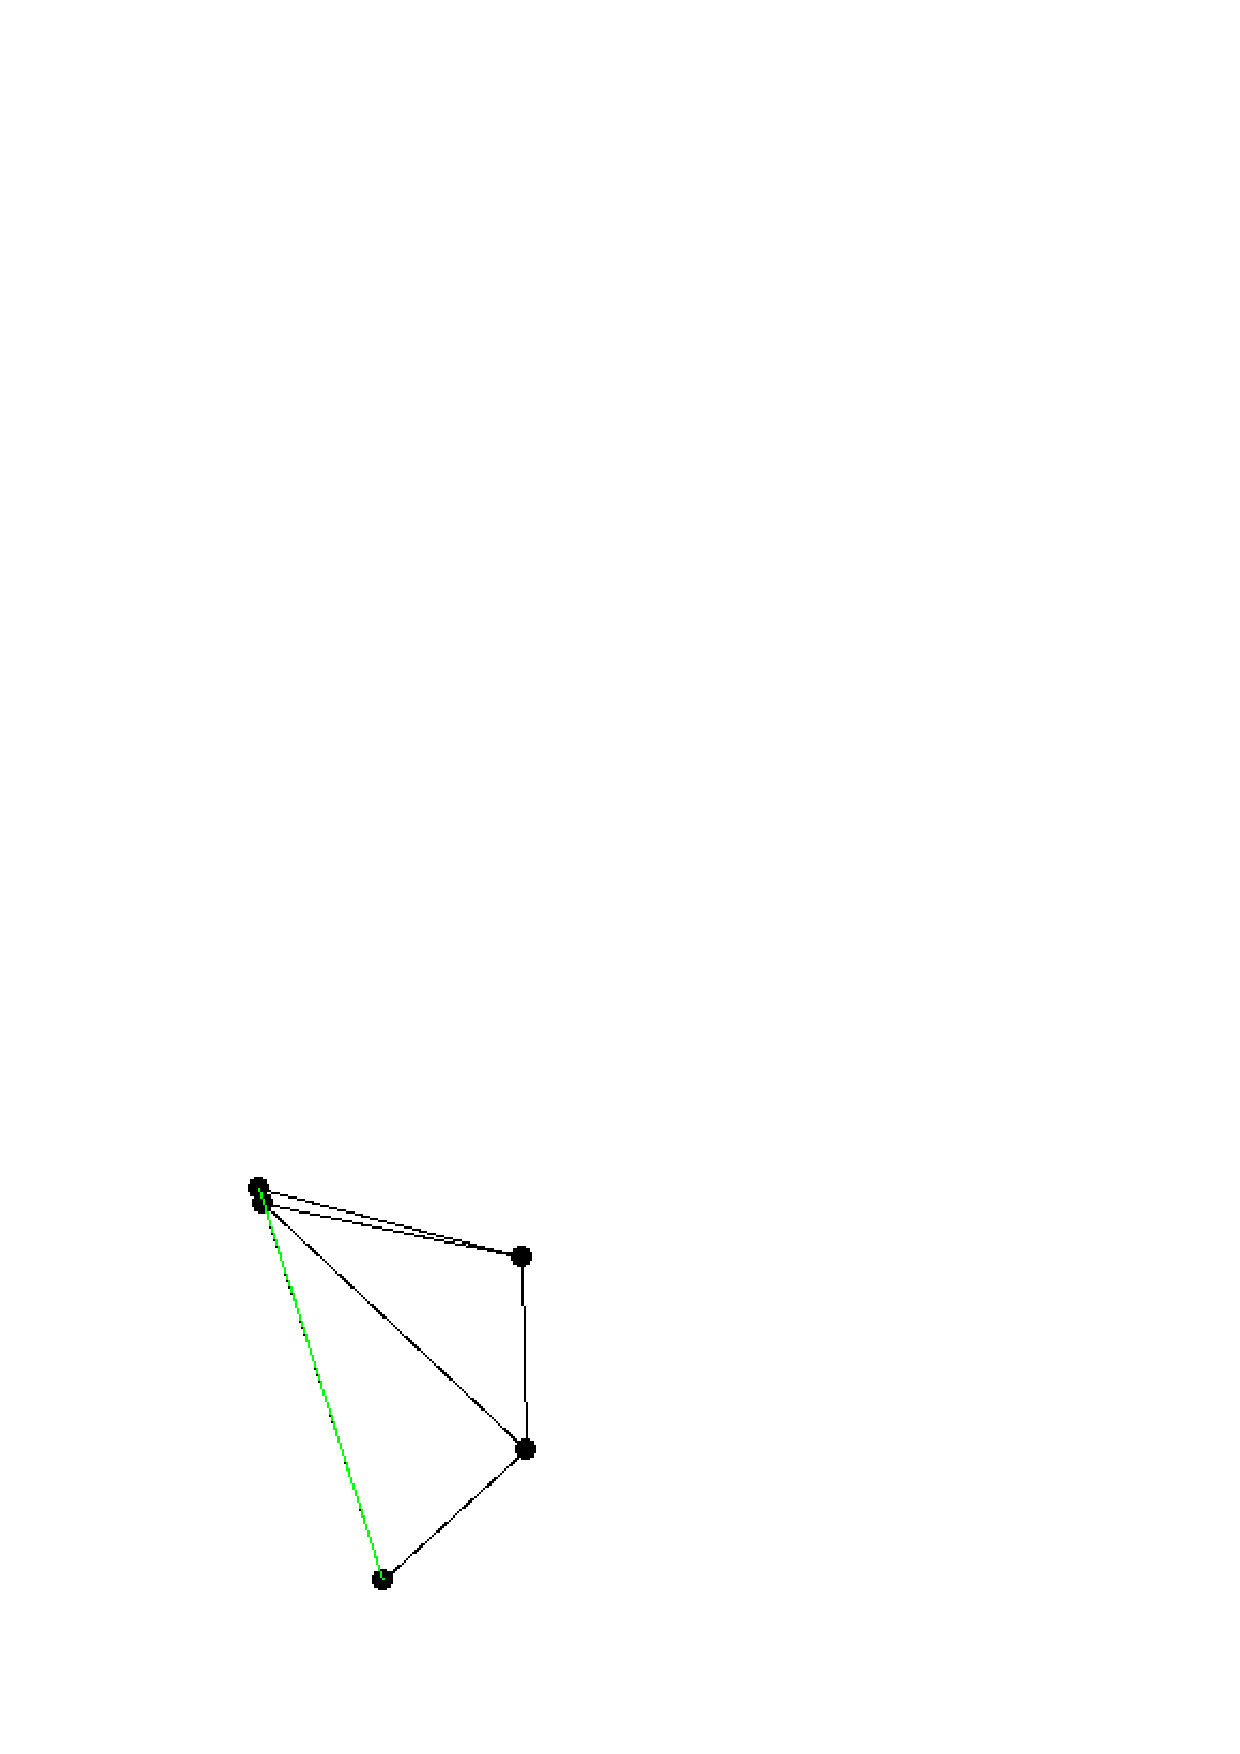
\includegraphics[ scale=.3]{Kinetic_data_structures/delaunay_shot_4_crop_pct}
6.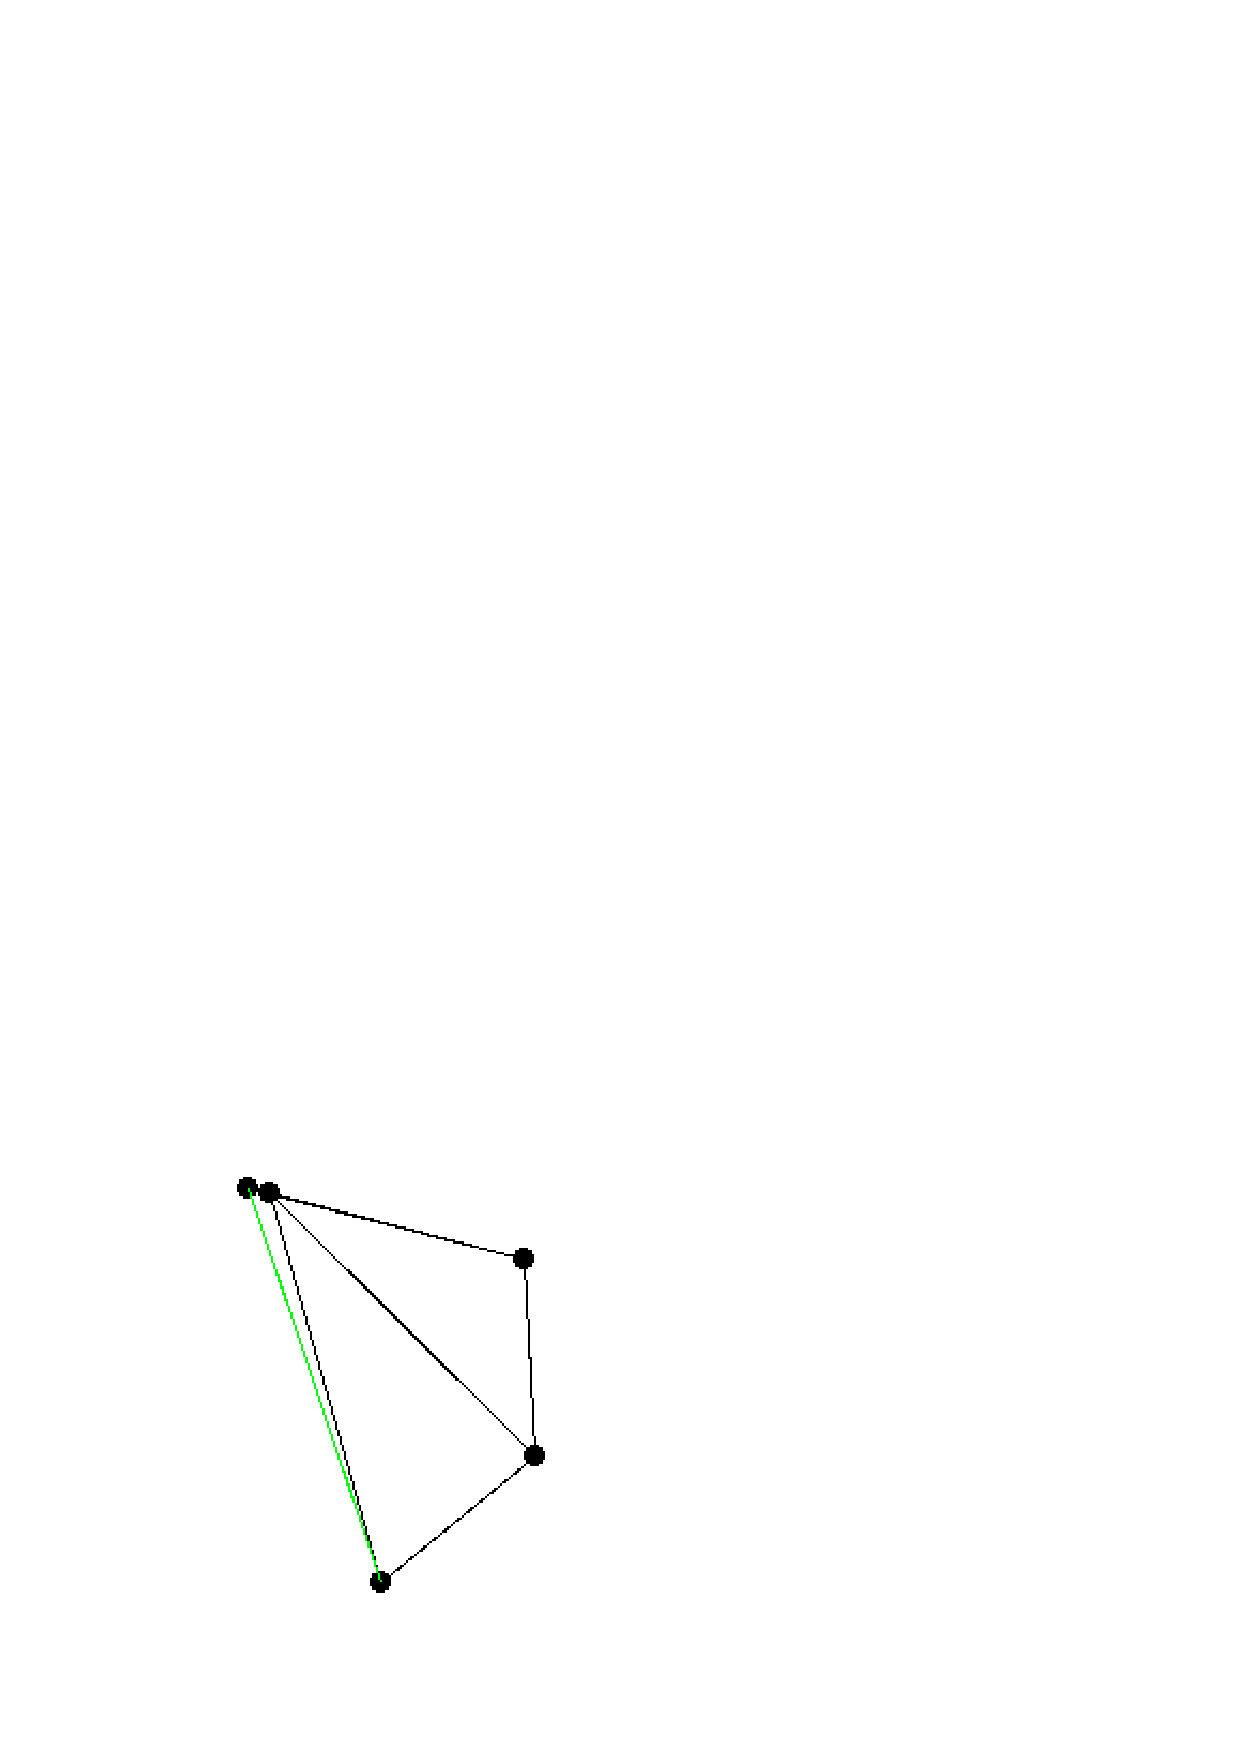
\includegraphics[ scale=.3]{Kinetic_data_structures/delaunay_shot_5_crop_pct}\\
7.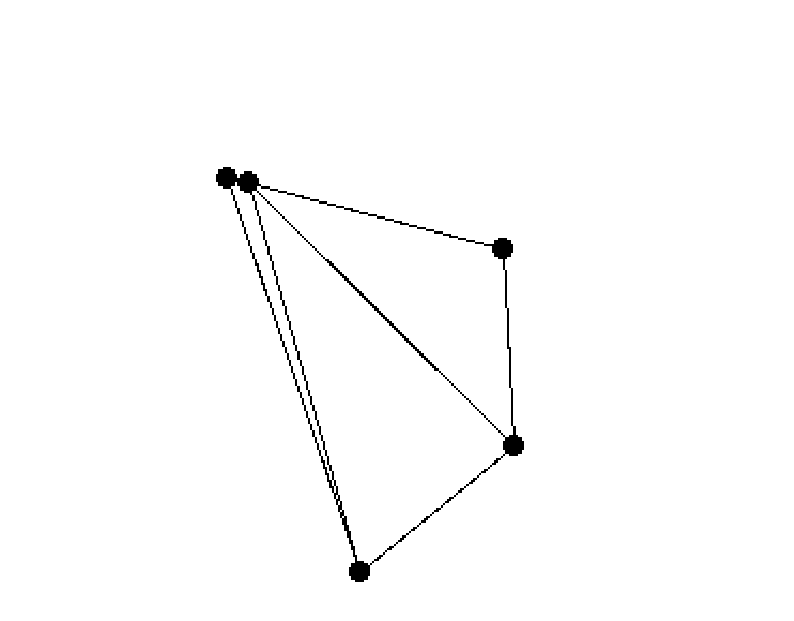
\includegraphics[ scale=.3]{Kinetic_data_structures/delaunay_shot_6_crop_pct}
8.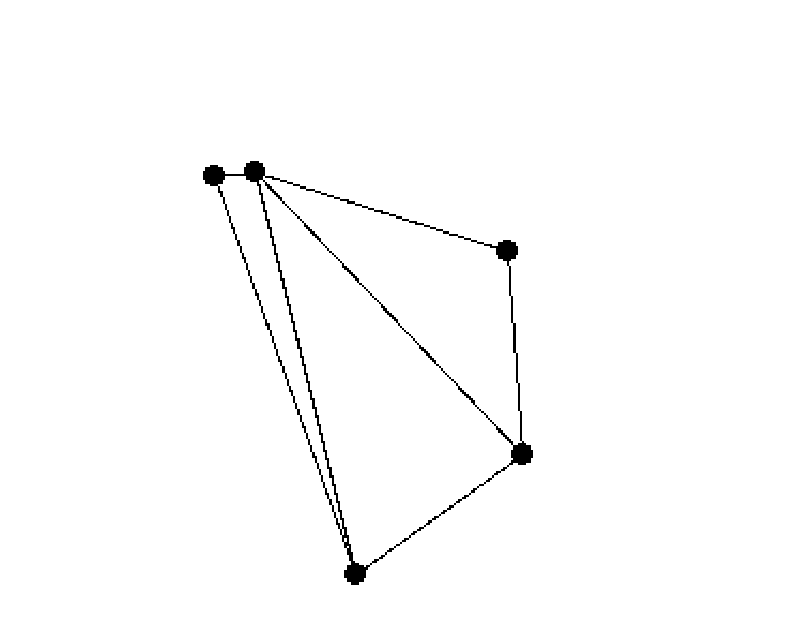
\includegraphics[ scale=.3]{Kinetic_data_structures/delaunay_shot_7_crop_pct}
\end{center}
\end{ccTexOnly}
\begin{ccHtmlOnly}
<imp border=1 src="./delaunay_shot_0.crop.gif" align=center alt="Frame 0">
<imp border=1 src="./delaunay_shot_1.crop.gif" align=center alt="Frame 1">
<imp border=1 src="./delaunay_shot_2.crop.gif" align=center alt="Frame 2">
<imp border=1 src="./delaunay_shot_3.crop.gif" align=center alt="Frame 3">
<imp border=1 src="./delaunay_shot_4.crop.gif" align=center alt="Frame 4">
<imp border=1 src="./delaunay_shot_5.crop.gif" align=center alt="Frame 5">
<imp border=1 src="./delaunay_shot_6.crop.gif" align=center alt="Frame 6">
<imp border=1 src="./delaunay_shot_7.crop.gif" align=center alt="Frame 7">
\end{ccHtmlOnly}
\caption{ \label{fig:delaunay_events} 
{\em Some events from a Delaunay triangulation kinetic data structure:} Before and after the first several events in a kinetic data structure is shown. The pictures are screen shots from demo/Kinetic\_data\_structures/Delaunay\_triangulation\_2.C. }
%\end{minipage}
%\end{center}
\end{figure*}


\label{fig:delaunay_2_usage_program}
\ccIncludeExampleCode{Kinetic_data_structures/Delaunay_triangulation_2.C}




\subsection{Extending Kinetic Data Structures\label{sec:kds_sweepline_example}}


Here we present a simple example that uses the
\ccc{Kinetic::Sort<Traits, Visitor>} kinetic data structure to compute
an arrangement of algebraic functions. It wraps the sorting data
structure and uses a visitor to monitor changes and map them to
corresponding features in the arrangement. To see an example using
this kinetic data structure read the example at
examples/Kinetic\_data\_structures/Kinetic_sweepline.cpp.

First we define the visitor class. An object of this type is passed to
the \ccc{Kinetic::Sort<Traits, Visitor>} data structure and turns
events into calls on the arrangement structure. This class has to be
defined externally since the arrangement will inherit from the sorting
structure.

\begin{ccExampleCode}
template <class Arrangement>
struct Arrangement_visitor: public Kinetic::Sort_visitor_base
{
  Arrangement_visitor(Arrangement *a):p_(a){}
  template <class Vertex_handle>
  void remove_vertex(Vertex_handle a) {
    p_->erase(a);
  }
  template <class Vertex_handle>
  void create_vertex(Vertex_handle a) {
    p_->insert(a);
  }
  template <class Vertex_handle>
  void after_swap(Vertex_handle a, Vertex_handle b) {
    p_->swap(a, b);
  }
  Arrangement *p_;
};

\end{ccExampleCode}

Now we define the actual arrangement data structure. 

\begin{ccExampleCode}

template <class TraitsT> 
class Planar_arrangement: 
  public Kinetic::Sort<TraitsT, 
		       Arrangement_visitor<Planar_arrangement<TraitsT> > > {
  typedef TraitsT Traits;
  typedef Planar_arrangement<TraitsT> This;
  typedef typename Kinetic::Sort<TraitsT,
				 Arrangement_visitor<This> > Sort;
  typedef Arrangement_visitor<This> Visitor;
  typedef typename Traits::Active_objects_table::Key Key;

public:
  typedef CGAL::Exact_predicates_inexact_constructions_kernel::Point_2 Approximate_point;
  typedef std::pair<int,int> Edge;
  typedef typename Sort::Vertex_handle Vertex_handle; 

  // Register this KDS with the MovingObjectTable and the Simulator
  Planar_arrangement(Traits tr): Sort(tr, Visitor(this)) {}

  Approximate_point vertex(int i) const
  {
    return approx_coords_[i];
  }

  size_t vertices_size() const
  {
    return approx_coords_.size();
  }

  typedef std::vector<Edge >::const_iterator Edges_iterator;
  Edges_iterator edges_begin() const
  {
    return edges_.begin();
  }
  Edges_iterator edges_end() const
  {
    return edges_.end();
  }

  void insert(Vertex_handle k) {
    last_points_[*k]=new_point(*k);
  }

  void swap(Vertex_handle a, Vertex_handle b) {
    int swap_point= new_point(*a);
    edges_.push_back(Edge(swap_point, last_points_[*a]));
    edges_.push_back(Edge(swap_point, last_points_[*b]));
    last_points_[*a]= swap_point;
    last_points_[*b]= swap_point;
  }

  void erase(Vertex_handle a) {
    edges_.push_back(Edge(last_points_[*a], new_point(*a)));
  }

  int new_point(typename Traits::Active_objects_table::Key k) {
    double tv= CGAL::to_double(Sort::traits().simulator_handle()->current_time());
    double dv= CGAL::to_double(Sort::traits().active_objects_table_handle()->at(k).x()(tv));
    approx_coords_.push_back(Approximate_point(tv, dv));
    return approx_coords_.size()-1;
  }

  std::vector<Approximate_point > approx_coords_;
  std::map<Key, int> last_points_;
  std::vector<Edge> edges_;

};
\end{ccExampleCode}

Finally, we have to set everything up. To do this we use some special
event classes: \ccc{Kinetic::Insert_event<ActiveObjectsTable>} and
\ccc{Kinetic::Erase_event<ActiveObjectsTable>}. These are events which
can be put in the event queue which either insert a primitive into the
set of active objects or remove it. Using these, we can allow curves
in the arrangement to begin or end in arbitrary places.
\begin{ccExampleCode}
typedef CGAL::Kinetic::Insert_event<Traits::Active_points_1_table> Insert_event;
typedef CGAL::Kinetic::Erase_event<Traits::Active_points_1_table> Erase_event;
do {
  NT begin, end;
  Point function;
  // initialize the function and the beginning and end somewhere
  tr.simulator_handle()->new_event(Time(begin),
			      Insert_event(function, tr.active_points_1_table_handle()));
  tr.simulator_handle()->new_event(Time(end),
				      Erase_event(Traits::Active_points_1_table::Key(num),
						  tr.active_points_1_table_handle()));
  ++num;
} while (true);
\end{ccExampleCode}
%%% Local Variables: 
%%% mode: latex
%%% TeX-master: t
%%% End: 



%%% Local Variables: 
%%% mode: latex
%%% TeX-master: t
%%% End: 



%%%%%%%%%%%%%%%%%%%%%%%%%%%%%%%%%%%%%%%%%%%%%%%%%%%%%%%%%%%%%%%%%%%%
\section{Architecture}
\label{sec:architecture}
%%%%%%%%%%%%%%%%%%%%%%%%%%%%%%%%%%%%%%%%%%%%%%%%%%%%%%%%%%%%%%%%%%%%


%%%%%%%%%%%%%%%%%%%%%%%%%%%%%%%%%%%%%%%%%%%%%%%%%%%%%%%%%%%%%%%%%%%%
\subsection{Overview}
\label{sec:architecture_overview}
%%%%%%%%%%%%%%%%%%%%%%%%%%%%%%%%%%%%%%%%%%%%%%%%%%%%%%%%%%%%%%%%%%%%

The framework is divided in to five main concepts as shown in Figure
\ref{fig:architecture}. These are all wrapped into a
\ccc{SimulatorTraits} concept, through which they are accessed to
preform various functions. Users of existing kinetic data structures will need to become familiar with the following two main concepts 
\begin{description}
\item[\ccc{Simulator}] a class that maintains the concept of time and a priority
  queue of the events. It is accessed from the \ccc{SimulationTraits} object using the \ccc{SimulationTraits::simulator_pointer()} method.
\item[\ccc{ActiveObjectsTable}] a container which stores kinetic geometric
  primitives and provides notifications when their trajectories
  change. The \ccc{SimulationTraits} creates an model of this concept
  called \ccc{SimulatorTraits::Moving_point_table} (assuming the
  primitives are points) which is accessible through the
  \ccc{SimulatorTraits::moving_point_table_pointer()} method.
\end{description}
Users who wish to implement kinetic data structures must become
familiar with a further two concepts:
\begin{description}
\item[\ccc{KineticKernel}]  a class which defines kinetic geometric primitives and
  predicates acting on them.
\item[\ccc{InstantaneousKernel}] a model of the CGAL kernel concept which allows static
  algorithms to act on a snapshot of the kinetic data structure.
\end{description}
The final main concept is that of the \ccc{FunctionKernel} a
computational kernel for representing and manipulating functions and
their roots. The \ccc{FunctionKernel}~ is provided by a separate
package and not discussed in detail here (other than the reference
page).

In a typical scenario using the framework, a model of
\ccc{SimulationTraits} is created and a number of geometric primitives
(e.g.\ points) are added to the
\ccc{SimulationTraits::Moving_point_table}. Then a kinetic data
structure, for example a two dimensional kinetic Delaunay
triangulation, is initialized and passed the \ccc{SimulationTraits}
object. The kinetic Delaunay triangulation extracts the trajectories
of the points from the \ccc{SimulationTraits::Moving_point_table} and
the current time from the \ccc{Simulator}. It then uses an instance of
an \ccc{InstantaneousKernel}, obtained from the \ccc{SimulationTraits}
to enable a static algorithm to compute the Delaunay triangulation of
the points at the current time. An instance of a \ccc{Kinetickernel}
is used to compute the \ccc{in_circle} certificate function for each
edge of the initial Delaunay triangulation (in order to verify that
the four points around the edge remain Delaunay). The kinetic data
structure requests that the \ccc{Simulator} solve each certificate
function and schedule an appropriate event. The \ccc{Simulator} uses
the \ccc{FunctionKernel} to compute and compare the roots of the
certificate functions.

Initialization is now complete and the kinetic data structure can be
run. Running consists of the \ccc{Simulator} finding the next event
and processing it until there are no more events. Here, processing an
event involves flipping an edge of the Delaunay triangulation and
computing five new event times (one for each of the edges around the
boundary of the quadralateral containing the edge and one for the edge
being flipped). The processing occurs via a callback from an object
representing an event to the kinetic Delaunay data structure.

If the trajectory of a primitive changes, for example it bounces
off a wall, then the \ccc{ActiveObjectsTable} notifies the kinetic Delaunay data
structure. The kinetic Delaunay data structure then updates all the
certificates of edges adjacent to faces containing the updated point and
reschedules those events with the \ccc{Simulator}.

A more detailed example will be discussed in
Section~\ref{sec:examples}. We will next discuss the main concepts in
order from most fundamental (and least exposed) to most exposed.

\begin{figure*}[htb]
\begin{ccTexOnly}
\begin{center}
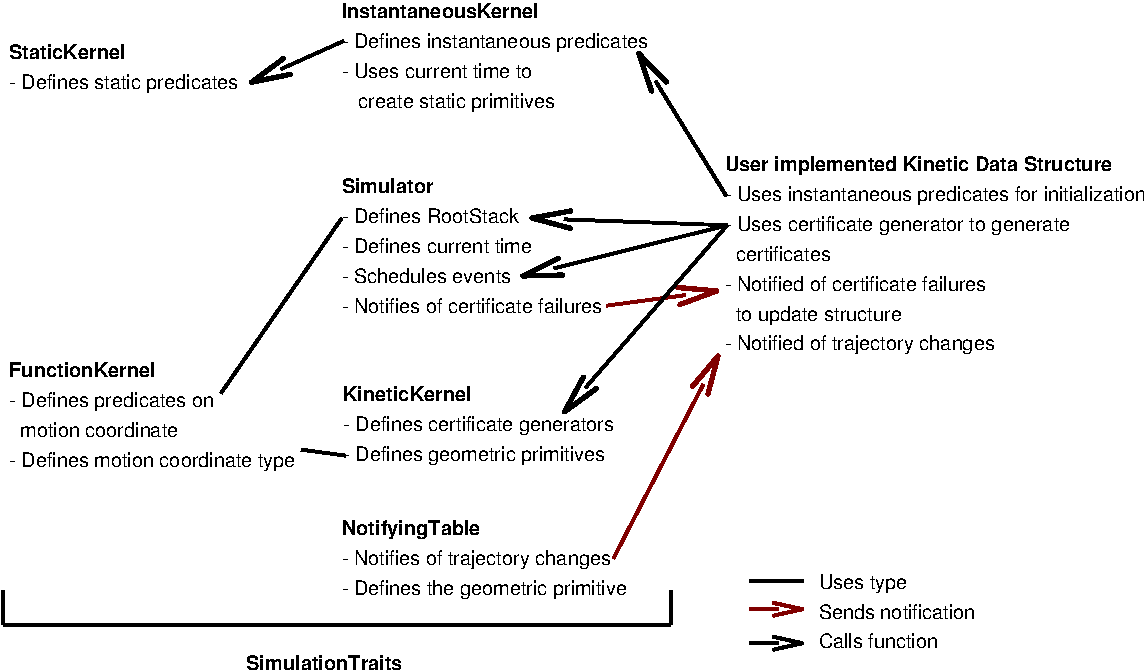
\includegraphics[ scale=.6]{Kinetic_data_structures/architecture_pct}
\end{center}
\end{ccTexOnly}
\begin{ccHtmlOnly}
<img border=1 src="./architecture_pct.gif" align=center alt="The architecture of the kinetic data structures package">
\end{ccHtmlOnly}
\caption{ \label{fig:architecture} 
{\em Framework architecture:} The main concepts and their relationships are shown. }
%\end{minipage}
%\end{center}
\end{figure*}



%%%%%%%%%%%%%%%%%%%%%%%%%%%%%%%%%%%%%%%%%%%%%%%%%%%%%%%%%%%%%%%%%%%%
\subsection{Kinetic primitives and predicates: the KineticKernel.}
\label{sec:kinetic_kernel}
%%%%%%%%%%%%%%%%%%%%%%%%%%%%%%%%%%%%%%%%%%%%%%%%%%%%%%%%%%%%%%%%%%%%

The \ccc{KineticKernel} is the kinetic analog of the CGAL
\ccc{Kernel}. It defines constant complexity kinetic geometric
primitives, kinetic predicates acting on them and constructions from
them. The short example in Section~\ref{sec:architecture_overview}
uses the \ccc{KineticKernel} to compute the \ccc{in\_circle}
certificate functions. We currently provide one model, namely
\ccc{CGAL::KDS::Cartesian_kinetic_kernel<FunctionKernel>}, which
defines two and three dimensional moving weighted and unweighted
points and the predicates necessary for Delaunay triangulations and
regular triangulations. The kernel provides the type \ccc{Function}
which plays the role of the \ccc{RT} in static
CGAL kernels and is the storage type for coordinates of kinetic
primitives. Algorithms request predicate functors from the kernel and
then apply these functors to kinetic primitives.

It is important to note that the \ccc{KineticKernel} does not have any notion of
finding roots of polynomials, of performing operations at the roots of
polynomials, or of static geometric concepts. The first and second are
restricted to the \ccc{FunctionKernel} and the \ccc{Simulator}
(Section~\ref{sec:simulator}). The third is handled by the \ccc{InstantaneousKernel} which
is discussed in the next section.

%%%%%%%%%%%%%%%%%%%%%%%%%%%%%%%%%%%%%%%%%%%%%%%%%%%%%%%%%%%%%%%%%%%%
\subsection{Connecting the kinetic and the static worlds: the InstantaneousKernel.}
\label{sec:instantaneous_kernel}
%%%%%%%%%%%%%%%%%%%%%%%%%%%%%%%%%%%%%%%%%%%%%%%%%%%%%%%%%%%%%%%%%%%%

The \ccc{InstantaneousKernel} allows other CGAL algorithms and data
structures to act on snapshots of a simulation. This ability is useful
for initializing and auditing kinietic data structures. A model of the
\ccc{InstantaneousKernel} concept proves a model of the CGAL
\ccc{Kernel} and works by computing the possition of each primitive in
the snapshot before performing the calculation requested by the static
algorithm.  For example, with the \ccc{InstantaneousKernel} we can use
the \ccc{Delaunay_triangulation_2<Traits, Tds>} to initialize a
kinetic Delaunay data structure and to insert new points into an
existing triangulation. In addition, the \ccc{InstantaneousKernel} can
be used to audit the kinetic data structure by comparing it to the
static data structure computed for that instant in time. We provide
two models, the
\ccc{CGAL::KDS::Cartesian_instantaneous_kernel<ActiveObjectsTable,
Kernel>} and
\ccc{CGAL::KDS::Regular_triangulation_instantaneous_traits<ActiveObjectsTable,
Kernel>}.

We are able to use this technique due to a couple of important
features of the CGAL architecture. First of all, the kernel is stored
as an object in CGAL data structures, so it can have state (for the
\ccc{InstantaneousKernel} the important state is the current time, and
the colection of trajectories). Secondly, predicates are not global
functions, instead they are functors that the algorithm requests from
the kernel. This means that they too, can have internal state. Then,
when an algorithm tries to compute a predicate, the predicate functor
asks the \ccc{InstantaneousKernel} to convert its input (handles to
kinetic geometric primitives) into static primitives and can then use
a predicate from a static CGAL kernel to properly compute the
predicate value.

Note that the time value used by our \ccc{InstantaneousKernel} model
must be support arithmetic operations. Some of the models of
\ccc{FunctionKernel} provide function root types which only support
comparisons, and consequently cannot be used here. In practice, this
is not a severe limitation, as discussed in the next section.

%%%%%%%%%%%%%%%%%%%%%%%%%%%%%%%%%%%%%%%%%%%%%%%%%%%%%%%%%%%%%%%%%%%%
\subsection{Tracking time: the Simulator.}
\label{sec:simulator}
%%%%%%%%%%%%%%%%%%%%%%%%%%%%%%%%%%%%%%%%%%%%%%%%%%%%%%%%%%%%%%%%%%%%

Running a kinetic data structure consists of repeatedly figuring out
when the next event occurs and processing it. This is the job of the
\ccc{Simulator}. It handles all event scheduling, descheduling and
processing and provides objects which can be used to determine when
certificate functions become invalid. Since events occur at the roots
of certificate functions (when the certificate function changes sign),
the \ccc{Root} type defined by a \ccc{FunctionKernel} is used to
represent time by the \ccc{Simulator}. In the example in
Section~\ref{sec:architecture_overview} the kinetic Delaunay data
structure requests that the \ccc{Simulator} determine when
\ccc{in\_circle} certificate functions become invalid and schedules an
\ccc{Event} with the \ccc{Simulator}. When the certificate fails, the
\ccc{Simulator} calls the \ccc{Event::process(Time)} method on the
\ccc{Event}. The framework provides one model of the \ccc{Simulator},
\ccc{CGAL::KDS::Simulator<FunctionKernel, EventQueue>}.

Note that the \ccc{CGAL::KDS::Simulator<FunctionKernel, EventQueue>}
is a object which is accessed by many other objects at run time (for
example, any running kinetic data structures, the graphical
interface). As a result, all access to it is through a reference
counted pointer, \ccc{CGAL::KDS::Simulator<FunctionKernel,
EventQueue>::Pointer}. This pointer can be safely stored. The
\ccc{Simulator} is created by the \ccc{SimulationTraits} and accessed
through the traits.

Our model of the \ccc{Simulator} is parameterized by a
\ccc{FunctionKernel} and a \ccc{EventQueue}. The former allows the
root stack (which allows enumeration of the roots of a polygon) and
root type to be changed, so numeric, exact or filtered exact
computation models can be used. The priority queue is by default a
queue which uses an interface with virtual functions to access the
events, allowing different kinetic data structures to use a single
queue. It can be replaced by a queue specialized for a particular
kinetic data structure if desired.

The \ccc{Root} concept is quite limited in which operations it
supports---it effectively only supports comparisons.  Roots cannot be
used in computations or as the time value in an
\ccc{InstantaneousKernel}. 

Two times, $t_0$ and $t_1$, are considered \textit{topologically
equivalent} if no roots occur in the interval $[t_0,t_1]$. The lack of
separating roots means that the function has the same sign over the
interval. This idea can be extended to a set of kinetic data
structures. When a simulation is running, if the time of the last event
which occurred, $t_{last}$, and the time of the next event,
$t_{next}$, are not equal, then the current combinatorial structures of
all of the kinetic data structures are valid over the entire interval
$(t_{last},t_{next})$. In addition there is a rational value of time,
$t_r$, which is topologically equivalent to all times in the
interval. Computations can be performed at $t_r$ since it can be
easily represented. This flexibility is used extensively in the \ccc{Simulator}.

When such a $t_r$ exists, the kinetic data structures are all
guaranteed to be valid (and the corresponding static data structure
non-degenerate) and so the data structure can be easily audited. The \ccc{Simulator} can
notify the kinetic data structures when this occurs and they can then
use an \ccc{InstantaneousKernel} to perform self-verification.

We can also use this idea to check the correctness of individual
certificates upon construction. We define a certificate to be invalid
when the certificate function is negative. As a result it
is an error, and a common sign of a bug in a kinetic data structure,
to construct a certificate function whose value is negative at the
time of construction. 
%
Unfortunately, the time of construction is
generally a root and this check cannot be performed easily. However,
we can find a time topologically equivalent to the current time for
that function (or discover if no such time exists) and evaluate the
function at that time. This is still a very expensive operation, but
faster than the alternative of using a real number type.

In addition, in order to properly handle two events occurring
simultaneously, the \ccc{Simulator} must check if the certificate function
being solved is zero at the current time. If it is zero, and negative
immediately afterwords, then the certificate fails immediately. This
can be checked in a similar manner.


%%%%%%%%%%%%%%%%%%%%%%%%%%%%%%%%%%%%%%%%%%%%%%%%%%%%%%%%%%%%%%%%%%%%
\subsection{Coordinating many kinetic data structures: the ActiveObjectsTable.}
\label{sec:moving_object_table}
%%%%%%%%%%%%%%%%%%%%%%%%%%%%%%%%%%%%%%%%%%%%%%%%%%%%%%%%%%%%%%%%%%%%

A framework for kinetic data structures needs to support updating the
trajectories of kinetic primitives, such as when a collision occurs,
and notification of the kinetic data structure of such changes. This
requirement is in contrast to static geometric data structures where
the geometric primitives never change and their representations are
often stored internally to the data structure. As a result, primitives
are stored in a centralized table and the data structures stores
\ccc{Key}s instead of the actual primitive. We provide one model of
such a table, \ccc{CGAL::KDS::Active_objects_vector<Object>}.

In the simple example presented in
Section~\ref{sec:architecture_overview}, the kinetic Delaunay
triangulation queries the \ccc{ActiveObjectsTable} for all the moving points on
initialization. Later, when the simulation is running, the
\ccc{ActiveObjectsTable} notifies the kinetic Delaunay data structure whenever a point's
trajectory changes.

More specifically, the \ccc{ActiveObjectsTable} allows multiple kinetic
data structures to access a set of kinetic geometric primitives of a
particular type and alerts the kinetic data structures when a new
primitive is added, one is removed, or a primitive's trajectory
changes. The user must specify what type of kinetic primitive a
particular instance of the \ccc{ActiveObjectsTable} model will contain
through a template argument. This type is exposed as the \ccc{Data}
type shown in the figure. To access an object, a \ccc{Key} which
uniquely identifies the object within this container and which has a
type specific to this container type is used.

The provided models of \ccc{SimulationTraits} each define a model of
\ccc{ActiveObjectsTable} containing points of appropriate
dimensionality. This type is called
\ccc{SimulationTraits::Moving_point_table} and accessed through
\ccc{SimulationTraits::moving_point_table_pointer()}. Like the
\ccc{Simulator} they \ccc{ActiveObjectsTable} models are explicitly shared
and accessed through reference counted pointers.

The \ccc{ActiveObjectsTable} uses a notification system which will be
briefly explained in Section~\ref{sec:misc} to notify interested
kinetic data structures when a set of changes to the primitives is
completed. The kinetic data structures must then request the keys of
the inserted, changed and erase objects from the
\ccc{ActiveObjectsTable} and handle them accordingly. We provide helper
classes to handle a number of common scenarios such as a kinetic data
structure which is incremental and can handle the changes of a single
object at a time (as is done in the example,
Figure~\ref{fig:example_program} in the appendix), or a kinetic data
structure which will rebuild all certificates any time any objects are
changed (which can be more efficient when many objects change at
once). The user can easily add other policies as needed.

The \ccc{ActiveObjectsTable} model provided will not meet the needs of
all users as there are many more specialized scenarios where a more
optimized handling of updates will be needed. The general structure of
the \ccc{ActiveObjectsTable} model can be extended to handle many such
cases. For example, if moving segments are used, then some kinetic
data structures will want to access each segment as an object, where
as others will only need to access the individual endpoints. This extra
capability can be added without forcing any changes to existing (point
based) kinetic data structures by adding methods to return modified
polygons in addition to those which return changed points.

When trajectory changes happen at rational time values, the
\ccc{ActiveObjectsTable} can check that the trajectories are
$C^0$-continuous. Unfortunately, the situation is much more
complicated for changes which occur at roots. In practice, motions can
be rounded off to nearby rational values without problem.

The \ccc{ActiveObjectsTable} only knows about one type of kinetic
primitive and has no concept of time, other kinetic primitives or
predicates. When a kinetic data structure handles an insertion, for
example, it must query the \ccc{Simulator} for an appropriate time
value and generate primitives using the \ccc{KineticKernel}. A more
detailed discussion of how to use the \ccc{ActiveObjectsTable} appears
in Section~\ref{sec:examples}.

%%%%%%%%%%%%%%%%%%%%%%%%%%%%%%%%%%%%%%%%%%%%%%%%%%%%%%%%%%%%%%%%%%%%
\subsection{Miscellaneous: graphical display, notification and reference management.}
\label{sec:misc}
%%%%%%%%%%%%%%%%%%%%%%%%%%%%%%%%%%%%%%%%%%%%%%%%%%%%%%%%%%%%%%%%%%%%

We describe some coding conventions used, graphical display,
notification and reference management support in the framework in the
following sections.


\subsubsection{Graphical display}

We provide a number of different classes to facilitate graphical
display and manipulation of kinetic data structures. There are two and
three dimensional user interfaces based on the Qt
(\ccc{CGAL::KDS::Qt_widget_2<Simulator>}) and Coin (\texttt{http://www.coin3d.org})
(\ccc{CGAL::KDS::QT_widget_3<Simulator>}) libraries,
respectively.  The graphical interfaces allows the simulations to be
start and stopped, events can be stepped through and time reversed.

We provide support for displaying two and three dimensional weighted
and unweighted point sets and two and three dimensional CGAL
triangulations. Other types can be easily added.

\subsubsection{Reference management}

A number of objects need to maintain pointers to other independent
objects. For example, each kinetic data structure must have access to
the \ccc{Simulator} so that it can schedule and deschedule events. These
pointers are all reference counted in order to guarantee that they are
always valid. We provide a standard reference counting pointer and
object base to facilitate this, namely \ccc{Ref_counted<Object>}.

Each shared object in the framework defines a type \ccc{Pointer} which is the
type for a reference counter pointer pointing to it. These should be
used for storing pointers to the objects in order to avoid dangling
pointers. In addition, many of the objects expect such pointers as
arguments.

\subsubsection{Runtime event passing}

Runtime events must be passed from \textit{notifiers}, namely the
\ccc{ActiveObjectsTable} and the \ccc{Simulator} to the kinetic data
structures to \textit{listeners}, such as a kinetic data structure
which needs to update itself when an event occurs These are passed
using a simple, standardized notification interface. To use
notifications, first defines a small proxy class which inherits from a
\ccc{Listener} base type provided by the notifier. The \ccc{Listener}
base class registers itself with the notifier on construction (and
unregisters itself on destruction).

When the some state of the notifier changes it, it calls the
\ccc{new_notification} method on the proxy object provided and passes
it a label corresponding to the name of the field that changed. The
proxy object can then call an appropriate method on the kinetic data
structure or other listening class.

In order to unregister on destruction, the \ccc{Listener} must store a
(reference counted) pointer to the object providing
notifications. This pointer can be accessed through the \ccc{notifier}
field. The \ccc{Listener} object stores a reference counted pointer to
the notifying object, while the notifying object stores a plain
pointer to the \ccc{Listener}. It can do this since the \ccc{Listener}
is guaranteed to unregister itself when it is destroyed. This avoids
circular reference counted pointers.



% Examples
\section{Examples}
\label{AABB_tree_section_examples}

\subsection{Triangles in a list}
In the following example a set of 3D triangles is stored in a list. The AABB primitive wraps a triangle and an iterator in the list. We computes the number of intersections between a 3D line and the input triangles, and the closest point from a query point to the input triangles.
\ccIncludeExampleCode{AABB_tree/AABB_triangle_3_example.cpp}

\subsection{Triangle facets of a polyhedral surface}
The following example computes the number of intersections between a 3D ray and a set of facets of a triangle polyhedral surface. The AABB primitive wraps a facet handle and generates on the fly a 3D triangle each time its object function is called.
\ccIncludeExampleCode{AABB_tree/AABB_polyhedron_facet_example.cpp}

\subsection{Segments in a list}
The following example computes the number of intersections between a 3D plane and a set of 3D segments. The segments are stored into a list, and the AABB primitive wraps a segment and an iterator in the list.
\ccIncludeExampleCode{AABB_tree/AABB_segment_3_example.cpp}

\subsection{Edges of a polyhedral surface}
The following example computes the number of intersections between a 3D plane and a set of edges of a triangle polyhedral surfaces. The AABB primitive wraps a halfedge handle and generates on the fly a 3D segment each time its object function is called..
\ccIncludeExampleCode{AABB_tree/AABB_polyhedron_edge_example.cpp}




% LocalWords:  Guibas Menelaos CGAL templated Expr KDSs deschedule
% LocalWords:  Karavelas
